\documentclass{article}\usepackage[]{graphicx}\usepackage[]{xcolor}
% maxwidth is the original width if it is less than linewidth
% otherwise use linewidth (to make sure the graphics do not exceed the margin)
\makeatletter
\def\maxwidth{ %
  \ifdim\Gin@nat@width>\linewidth
    \linewidth
  \else
    \Gin@nat@width
  \fi
}
\makeatother

\definecolor{fgcolor}{rgb}{0.345, 0.345, 0.345}
\newcommand{\hlnum}[1]{\textcolor[rgb]{0.686,0.059,0.569}{#1}}%
\newcommand{\hlsng}[1]{\textcolor[rgb]{0.192,0.494,0.8}{#1}}%
\newcommand{\hlcom}[1]{\textcolor[rgb]{0.678,0.584,0.686}{\textit{#1}}}%
\newcommand{\hlopt}[1]{\textcolor[rgb]{0,0,0}{#1}}%
\newcommand{\hldef}[1]{\textcolor[rgb]{0.345,0.345,0.345}{#1}}%
\newcommand{\hlkwa}[1]{\textcolor[rgb]{0.161,0.373,0.58}{\textbf{#1}}}%
\newcommand{\hlkwb}[1]{\textcolor[rgb]{0.69,0.353,0.396}{#1}}%
\newcommand{\hlkwc}[1]{\textcolor[rgb]{0.333,0.667,0.333}{#1}}%
\newcommand{\hlkwd}[1]{\textcolor[rgb]{0.737,0.353,0.396}{\textbf{#1}}}%
\let\hlipl\hlkwb

\usepackage{framed}
\makeatletter
\newenvironment{kframe}{%
 \def\at@end@of@kframe{}%
 \ifinner\ifhmode%
  \def\at@end@of@kframe{\end{minipage}}%
  \begin{minipage}{\columnwidth}%
 \fi\fi%
 \def\FrameCommand##1{\hskip\@totalleftmargin \hskip-\fboxsep
 \colorbox{shadecolor}{##1}\hskip-\fboxsep
     % There is no \\@totalrightmargin, so:
     \hskip-\linewidth \hskip-\@totalleftmargin \hskip\columnwidth}%
 \MakeFramed {\advance\hsize-\width
   \@totalleftmargin\z@ \linewidth\hsize
   \@setminipage}}%
 {\par\unskip\endMakeFramed%
 \at@end@of@kframe}
\makeatother

\definecolor{shadecolor}{rgb}{.97, .97, .97}
\definecolor{messagecolor}{rgb}{0, 0, 0}
\definecolor{warningcolor}{rgb}{1, 0, 1}
\definecolor{errorcolor}{rgb}{1, 0, 0}
\newenvironment{knitrout}{}{} % an empty environment to be redefined in TeX

\usepackage{alltt}
\usepackage[margin=1.0in]{geometry} % To set margins
\usepackage{amsmath}  % This allows me to use the align functionality.
                      % If you find yourself trying to replicate
                      % something you found online, ensure you're
                      % loading the necessary packages!
\usepackage{amsfonts} % Math font
\usepackage{fancyvrb}
\usepackage{hyperref} % For including hyperlinks
\usepackage[shortlabels]{enumitem}% For enumerated lists with labels specified
                                  % We had to run tlmgr_install("enumitem") in R
\usepackage{float}    % For telling R where to put a table/figure
\usepackage{natbib}        %For the bibliography
\bibliographystyle{apalike}%For the bibliography
\IfFileExists{upquote.sty}{\usepackage{upquote}}{}
\begin{document}


\cite{Kasdin25} show that dopamine in the brains of young zebra finches acts as 
a learning signal, increasing when they sing closer to their adult song and 
decreasing when they sing further away, effectively guiding their vocal 
development through trial-and-error. This suggests that complex natural 
behaviors, like learning to sing, are shaped by dopamine-driven reinforcement 
learning, similar to how artificial intelligence learns. You can find the 
paper at this link:
\href{https://www.nature.com/articles/s41586-025-08729-1}{{https://www.nature.com/articles/s41586-025-08729-1}.}.

Note they measure dopamine using fibre photometry, changes in the fluorescence
indicate dopamine changes in realtime. Their specific measurement considers 
changes in flourescence in 100-ms windows between 200 and 300 ms from the start 
of singing, averaged across development.

\begin{enumerate}
%%%%%%%%%%%%%%%%%%%%%%%%%%%%%%%%%%%%%%%%%%%%%%%%%%%%%%%%%%%%%%%%%
% CONDUCT A POWER ANALYSIS
%%%%%%%%%%%%%%%%%%%%%%%%%%%%%%%%%%%%%%%%%%%%%%%%%%%%%%%%%%%%%%%%%
\item Using the \texttt{pwr} package for \texttt{R} \citep{pwr},
conduct a power analysis. How many observations would the researchers 
need to detect a moderate-to-large effect ($d=0.65$) when using 
$\alpha=0.05$ and default power (0.80) for a two-sided one sample 
$t$ test.

\begin{knitrout}
\definecolor{shadecolor}{rgb}{0.969, 0.969, 0.969}\color{fgcolor}\begin{kframe}
\begin{alltt}
\hlkwd{library}\hldef{(pwr)}

\hldef{alpha} \hlkwb{=} \hlnum{0.05}

\hldef{pwr.testing} \hlkwb{<-} \hlkwd{pwr.t.test}\hldef{(}\hlkwc{d}\hldef{=}\hlnum{0.65}\hldef{,} \hlkwc{sig.level} \hldef{= alpha,} \hlkwc{power} \hldef{=} \hlnum{0.80}\hldef{,}
                          \hlkwc{type} \hldef{=} \hlsng{"one.sample"}\hldef{,} \hlkwc{alternative} \hldef{=} \hlsng{"two.sided"}\hldef{)}
\hldef{(pwr.testing}\hlopt{$}\hldef{n)}
\end{alltt}
\begin{verbatim}
## [1] 20.58039
\end{verbatim}
\end{kframe}
\end{knitrout}

\textbf{Solution:} The number of observations needed to achieve the defined parameters is $n = 20.58039$. To obtain this value of $n$, I used the \verb|pwr.t.test()| function from the \textbf{pwr} package. I was able to plug in all the given parameters into this function to calculate the number of observations needed.
%%%%%%%%%%%%%%%%%%%%%%%%%%%%%%%%%%%%%%%%%%%%%%%%%%%%%%%%%%%%%%%%%
% COLLECT DATA
%%%%%%%%%%%%%%%%%%%%%%%%%%%%%%%%%%%%%%%%%%%%%%%%%%%%%%%%%%%%%%%%%
\item Click the link to go to the paper. Find the source data for 
Figure 2. Download the Excel file. Describe what you needed to
do to collect the data for Figure 2(g). Note that you only need the 
\texttt{closer\_vals} and \texttt{further\_vals}. Ensure to 
\texttt{mutate()} the data to get a difference 
(e.g., \texttt{closer\_vals - further\_vals}).

\begin{knitrout}
\definecolor{shadecolor}{rgb}{0.969, 0.969, 0.969}\color{fgcolor}\begin{kframe}
\begin{alltt}
\hlkwd{library}\hldef{(xtable)}
\hlkwd{library}\hldef{(tidyverse)}

\hldef{closer.vals} \hlkwb{<-} \hlkwd{read_csv}\hldef{(}\hlsng{"Closer_vals.csv"}\hldef{)}

\hldef{farther.vals} \hlkwb{<-} \hlkwd{read_csv}\hldef{(}\hlsng{"Farther_vals.csv"}\hldef{)}

\hldef{figure2G.data} \hlkwb{<-} \hlkwd{tibble}\hldef{(}\hlkwc{closer_vals} \hldef{= closer.vals}\hlopt{$}\hldef{Closer_vals,}
                    \hlkwc{farther_vals} \hldef{= farther.vals}\hlopt{$}\hldef{Farther_vals) |>}
  \hlkwd{mutate}\hldef{(}\hlkwc{difference} \hldef{= closer_vals} \hlopt{-} \hldef{farther_vals)}

\hlkwd{xtable}\hldef{(figure2G.data)}
\end{alltt}
\end{kframe}
\end{knitrout}

\begin{table}[ht]
\centering
\begin{tabular}{rrrr}
\hline
observation & closer\_vals & farther\_vals & difference \\
\hline
1 & 0.28 & -0.19 & 0.47 \\
2 & 0.08 & -0.03 & 0.11 \\
3 & 0.13 & -0.19 & 0.32 \\
4 & 0.04 & -0.07 & 0.11 \\
5 & 0.15 & -0.09 & 0.23 \\
6 & 0.20 & -0.16 & 0.36 \\
7 & 0.16 & -0.31 & 0.47 \\
8 & 0.18 & -0.16 & 0.34 \\
9 & 0.13 & -0.13 & 0.26 \\
10 & 0.10 & -0.05 & 0.15 \\
11 & 0.33 & -0.60 & 0.93 \\
12 & 0.17 & -0.24 & 0.41 \\
13 & 0.07 & -0.12 & 0.20 \\
14 & 0.00 & -0.13 & 0.13 \\
15 & 0.00 & -0.04 & 0.04 \\
16 & 0.09 & -0.24 & 0.33 \\
17 & 0.26 & -0.34 & 0.61 \\
18 & 0.28 & -0.31 & 0.59 \\
19 & 0.07 & -0.18 & 0.25 \\
20 & 0.15 & -0.07 & 0.23 \\
21 & 0.27 & -0.34 & 0.61 \\
22 & 0.15 & -0.19 & 0.34 \\
23 & 0.10 & -0.20 & 0.30 \\
24 & 0.19 & -0.31 & 0.50 \\
25 & 0.34 & -0.35 & 0.69 \\
\hline
\end{tabular}
\caption{Table of \texttt{closer\_vals}, \texttt{farther\_vals}, and \texttt{difference} for each observation.}
\label{table1}
\end{table}

\textbf{Information:} This information was tablulated through the \textbf{R xtable} package.
\newpage

%%%%%%%%%%%%%%%%%%%%%%%%%%%%%%%%%%%%%%%%%%%%%%%%%%%%%%%%%%%%%%%%%
% SUMMARIZE DATA
%%%%%%%%%%%%%%%%%%%%%%%%%%%%%%%%%%%%%%%%%%%%%%%%%%%%%%%%%%%%%%%%%
\item Summarize the data.
\begin{enumerate}
  \item Summarize the further data. Do the data suggest that
   dopamine in the brains of young zebra finches decreases when
   they sing further away?
\begin{knitrout}
\definecolor{shadecolor}{rgb}{0.969, 0.969, 0.969}\color{fgcolor}\begin{kframe}
\begin{alltt}
\hldef{farther.summary} \hlkwb{<-} \hlkwd{summarize}\hldef{(figure2G.data,}
                            \hlkwc{mean} \hldef{=} \hlkwd{mean}\hldef{(farther_vals),}
                            \hlkwc{variance} \hldef{=} \hlkwd{var}\hldef{(farther_vals),}
                            \hlkwc{median} \hldef{=} \hlkwd{median}\hldef{(farther_vals),}
                            \hlkwc{IQR} \hldef{=} \hlkwd{IQR}\hldef{(farther_vals),}
                            \hlkwc{skew} \hldef{=} \hlkwd{skewness}\hldef{(farther_vals),}
                            \hlkwc{e.kurt} \hldef{=} \hlkwd{kurtosis}\hldef{(farther_vals),}
                            \hlkwc{min} \hldef{=} \hlkwd{min}\hldef{(farther_vals),}
                            \hlkwc{max} \hldef{=} \hlkwd{max}\hldef{(farther_vals))}
\hlkwd{xtable}\hldef{(farther.summary)}
\end{alltt}
\end{kframe}
\end{knitrout}

As can be seen in Table 2, both the mean and median statistics are negative which suggests that as young zebra finches are further away from the adult songs they experience a decrease in dopamine levels. Both the minimum and maximum values being negative also suggests that in all cases young zebra finches experience a decrease in dopamine levels.

\begin{table}[ht]
\centering
\begin{tabular}{rrrrrrrrr}
  \hline
mean & variance & median & IQR & skew & e.kurt & min & max \\ 
  \hline
-0.20 & 0.02 & -0.19 & 0.19 & -1.04 & 1.19 & -0.60 & -0.03 \\ 
   \hline
\end{tabular}
\caption{Summary Statistics Regarding Farther Data.}
\label{table2}
\end{table}

   \item Summarize the closer data. Do the data suggest that
   dopamine in the brains of young zebra finches increases when
   they sing closer to their adult song?

\begin{knitrout}
\definecolor{shadecolor}{rgb}{0.969, 0.969, 0.969}\color{fgcolor}\begin{kframe}
\begin{alltt}
\hldef{closer.summary} \hlkwb{<-} \hlkwd{summarize}\hldef{(figure2G.data,}
                             \hlkwc{mean} \hldef{=} \hlkwd{mean}\hldef{(closer_vals),}
                             \hlkwc{variance} \hldef{=} \hlkwd{var}\hldef{(closer_vals),}
                             \hlkwc{median} \hldef{=} \hlkwd{median}\hldef{(closer_vals),}
                             \hlkwc{IQR} \hldef{=} \hlkwd{IQR}\hldef{(closer_vals),}
                             \hlkwc{skew} \hldef{=} \hlkwd{skewness}\hldef{(closer_vals),}
                             \hlkwc{e.kurt} \hldef{=} \hlkwd{kurtosis}\hldef{(closer_vals),}
                             \hlkwc{min} \hldef{=} \hlkwd{min}\hldef{(closer_vals),}
                             \hlkwc{max} \hldef{=} \hlkwd{max}\hldef{(closer_vals))}
\hlkwd{xtable}\hldef{(closer.summary)}
\end{alltt}
\end{kframe}
\end{knitrout}

As can be seen in Table 3, both the mean and median statistics are positive which suggests that as young zebra finches are closer to the adult songs they experience an increase in dopamine levels. The minimum and maximum values also supplement the idea that as young zebra finches sing closer to the adult songs they experience an increase in dopamine levels because both statistics are postive.

\begin{table}[ht]
\centering
\begin{tabular}{rrrrrrrrr}
  \hline
mean & variance & median & IQR & skew & e.kurt & min & max \\ 
  \hline
0.16 & 0.01 & 0.15 & 0.11 & 0.30 & -0.86 & 0.00 & 0.34 \\ 
   \hline
\end{tabular}
\caption{Summary Statistics Regarding Closer Data.}
\label{table3}
\end{table}

  \item Summarize the paired differences. Do the data suggest
  that there is a difference between dopamine in the brains of
  young zebra finches when they sing further away compared to 
  closer to their adult song?

\begin{knitrout}
\definecolor{shadecolor}{rgb}{0.969, 0.969, 0.969}\color{fgcolor}\begin{kframe}
\begin{alltt}
\hldef{difference.summary} \hlkwb{<-} \hlkwd{summarize}\hldef{(figure2G.data,}
                            \hlkwc{mean} \hldef{=} \hlkwd{mean}\hldef{(difference),}
                            \hlkwc{variance} \hldef{=} \hlkwd{var}\hldef{(difference),}
                            \hlkwc{median} \hldef{=} \hlkwd{median}\hldef{(difference),}
                            \hlkwc{IQR} \hldef{=} \hlkwd{IQR}\hldef{(difference),}
                            \hlkwc{skew} \hldef{=} \hlkwd{skewness}\hldef{(difference),}
                            \hlkwc{e.kurt} \hldef{=} \hlkwd{kurtosis}\hldef{(difference),}
                            \hlkwc{min} \hldef{=} \hlkwd{min}\hldef{(difference),}
                            \hlkwc{max} \hldef{=} \hlkwd{max}\hldef{(difference))}
\hlkwd{xtable}\hldef{(difference.summary)}
\end{alltt}
\end{kframe}
\end{knitrout}

\begin{table}[ht]
\centering
\begin{tabular}{rrrrrrrrr}
  \hline
mean & variance & median & IQR & skew & e.kurt & min & max \\ 
  \hline
0.36 & 0.04 & 0.33 & 0.24 & 0.77 & 0.13 & 0.04 & 0.93 \\ 
   \hline
\end{tabular}
\caption{Summary Statistics Regarding The Difference Between Closer Data and Farther Data.}
\label{table4}
\end{table}

\end{enumerate}
%%%%%%%%%%%%%%%%%%%%%%%%%%%%%%%%%%%%%%%%%%%%%%%%%%%%%%%%%%%%%%%%%
% CONDUCT THE TESTS
%%%%%%%%%%%%%%%%%%%%%%%%%%%%%%%%%%%%%%%%%%%%%%%%%%%%%%%%%%%%%%%%%
\item Conduct the inferences they do in the paper. Make sure to report the results
a little more comprehensively -- that is your parenthetical should look something
like: ($t=23.99$, $p<0.0001$; $g=1.34$; 95\% CI: 4.43, 4.60).\\
\textbf{Note:} Your numbers may vary slightly as they performed some unclear
correction of their $p$-values. I'm waiting to hear back from them via email!

\textbf{NOTE:} To accomplish the tasks in part 4, we used the \verb|hedges_g(), t.test(), and interpret_hedges_g()| from the \texttt{effectsize} \citep(effectsize) package.

\begin{enumerate}
  \item ``The close responses differed significantly from 0 ($p=1.63 \times 10^{-8}$).''
  
\begin{knitrout}
\definecolor{shadecolor}{rgb}{0.969, 0.969, 0.969}\color{fgcolor}\begin{kframe}
\begin{alltt}
\hldef{mu0} \hlkwb{<-} \hlnum{0}
\hldef{x.close} \hlkwb{<-} \hldef{figure2G.data}\hlopt{$}\hldef{closer_vals}

\hlkwd{hedges_g}\hldef{(}\hlkwc{x} \hldef{= x.close,} \hlkwc{mu} \hldef{= mu0,} \hlkwc{alternative} \hldef{=} \hlsng{"greater"}\hldef{)}
\end{alltt}
\begin{verbatim}
## Hedges' g |      95% CI
## -----------------------
## 1.61      | [1.10, Inf]
## 
## - One-sided CIs: upper bound fixed at [Inf].
\end{verbatim}
\begin{alltt}
\hlkwd{interpret_hedges_g}\hldef{(}\hlnum{1.61}\hldef{)}
\end{alltt}
\begin{verbatim}
## [1] "large"
## (Rules: cohen1988)
\end{verbatim}
\begin{alltt}
\hlkwd{t.test}\hldef{(}\hlkwc{x} \hldef{= x.close,} \hlkwc{mu} \hldef{= mu0,} \hlkwc{alternative} \hldef{=} \hlsng{"greater"}\hldef{)}
\end{alltt}
\begin{verbatim}
## 
## 	One Sample t-test
## 
## data:  x.close
## t = 8.3024, df = 24, p-value = 8.132e-09
## alternative hypothesis: true mean is greater than 0
## 95 percent confidence interval:
##  0.1240301       Inf
## sample estimates:
## mean of x 
## 0.1562231
\end{verbatim}
\begin{alltt}
\hldef{(CI.upper} \hlkwb{<-} \hlkwd{t.test}\hldef{(}\hlkwc{x} \hldef{= x.close,}
                    \hlkwc{mu} \hldef{= mu0,}
                    \hlkwc{alternative} \hldef{=} \hlsng{"two.sided"}\hldef{)}\hlopt{$}\hldef{conf.int[}\hlnum{2}\hldef{])}
\end{alltt}
\begin{verbatim}
## [1] 0.1950586
\end{verbatim}
\end{kframe}
\end{knitrout}

\textbf{Solution:} ($t=8.3024$, $p<0.0001$; $g=1.61$; 95\% CI: 0.1240, 0.1951)
  
  \item ``The far responses differed significantly from 0 ($p=5.17 \times 10^{-8}$).''
  
\begin{knitrout}
\definecolor{shadecolor}{rgb}{0.969, 0.969, 0.969}\color{fgcolor}\begin{kframe}
\begin{alltt}
\hldef{mu0} \hlkwb{<-} \hlnum{0}
\hldef{x.far} \hlkwb{<-} \hldef{figure2G.data}\hlopt{$}\hldef{farther_vals}

\hlkwd{hedges_g}\hldef{(}\hlkwc{x} \hldef{= x.far,} \hlkwc{mu} \hldef{= mu0,} \hlkwc{alternative} \hldef{=} \hlsng{"less"}\hldef{)}
\end{alltt}
\begin{verbatim}
## Hedges' g |        95% CI
## -------------------------
## -1.51     | [-Inf, -1.02]
## 
## - One-sided CIs: lower bound fixed at [-Inf].
\end{verbatim}
\begin{alltt}
\hlkwd{interpret_hedges_g}\hldef{(}\hlopt{-}\hlnum{1.51}\hldef{)}
\end{alltt}
\begin{verbatim}
## [1] "large"
## (Rules: cohen1988)
\end{verbatim}
\begin{alltt}
\hlkwd{t.test}\hldef{(}\hlkwc{x} \hldef{= x.far,} \hlkwc{mu} \hldef{= mu0,} \hlkwc{alternative} \hldef{=} \hlsng{"less"}\hldef{)}
\end{alltt}
\begin{verbatim}
## 
## 	One Sample t-test
## 
## data:  x.far
## t = -7.778, df = 24, p-value = 2.587e-08
## alternative hypothesis: true mean is less than 0
## 95 percent confidence interval:
##        -Inf -0.1581322
## sample estimates:
##  mean of x 
## -0.2027244
\end{verbatim}
\begin{alltt}
\hldef{(CI.lower} \hlkwb{<-} \hlkwd{t.test}\hldef{(}\hlkwc{x} \hldef{= x.far,}
                    \hlkwc{mu} \hldef{= mu0,}
                    \hlkwc{alternative} \hldef{=} \hlsng{"two.sided"}\hldef{)}\hlopt{$}\hldef{conf.int[}\hlnum{1}\hldef{])}
\end{alltt}
\begin{verbatim}
## [1] -0.2565176
\end{verbatim}
\end{kframe}
\end{knitrout}

\textbf{Solution:} ($t=-7.778$, $p<0.0001$; $g=-1.51$; 95\% CI: -0.2565, -0.1581)

  \item ``The difference between populations was significant ($p=1.04 \times10^{-8}$).''
  
\begin{knitrout}
\definecolor{shadecolor}{rgb}{0.969, 0.969, 0.969}\color{fgcolor}\begin{kframe}
\begin{alltt}
\hldef{mu0} \hlkwb{<-} \hlnum{0}
\hldef{x.difference} \hlkwb{<-} \hldef{figure2G.data}\hlopt{$}\hldef{difference}

\hlkwd{hedges_g}\hldef{(}\hlkwc{x} \hldef{= x.difference,} \hlkwc{mu} \hldef{= mu0,} \hlkwc{alternative} \hldef{=} \hlsng{"two.sided"}\hldef{)}
\end{alltt}
\begin{verbatim}
## Hedges' g |       95% CI
## ------------------------
## 1.65      | [1.04, 2.24]
\end{verbatim}
\begin{alltt}
\hlkwd{interpret_hedges_g}\hldef{(}\hlnum{1.65}\hldef{)}
\end{alltt}
\begin{verbatim}
## [1] "large"
## (Rules: cohen1988)
\end{verbatim}
\begin{alltt}
\hlkwd{t.test}\hldef{(}\hlkwc{x}\hldef{=x.difference,} \hlkwc{mu} \hldef{= mu0,} \hlkwc{alternative} \hldef{=} \hlsng{"two.sided"}\hldef{)}
\end{alltt}
\begin{verbatim}
## 
## 	One Sample t-test
## 
## data:  x.difference
## t = 8.5109, df = 24, p-value = 1.037e-08
## alternative hypothesis: true mean is not equal to 0
## 95 percent confidence interval:
##  0.2719028 0.4459921
## sample estimates:
## mean of x 
## 0.3589475
\end{verbatim}
\end{kframe}
\end{knitrout}

\textbf{Solution:} ($t=8.5109$, $p<0.0001$; $g=1.65$; 95\% CI: 0.272, 0.446)
\end{enumerate}
%%%%%%%%%%%%%%%%%%%%%%%%%%%%%%%%%%%%%%%%%%%%%%%%%%%%%%%%%%%%%%%%%
% CONDUCT THE TESTS
%%%%%%%%%%%%%%%%%%%%%%%%%%%%%%%%%%%%%%%%%%%%%%%%%%%%%%%%%%%%%%%%%
\item Reverse engineer the hypothesis test plot from Lecture 20 to create accurate
hypothesis testing plots for each part of the previous question.
\begin{enumerate}
  \item Question 4, part(a).
\begin{figure}[H]
\centering
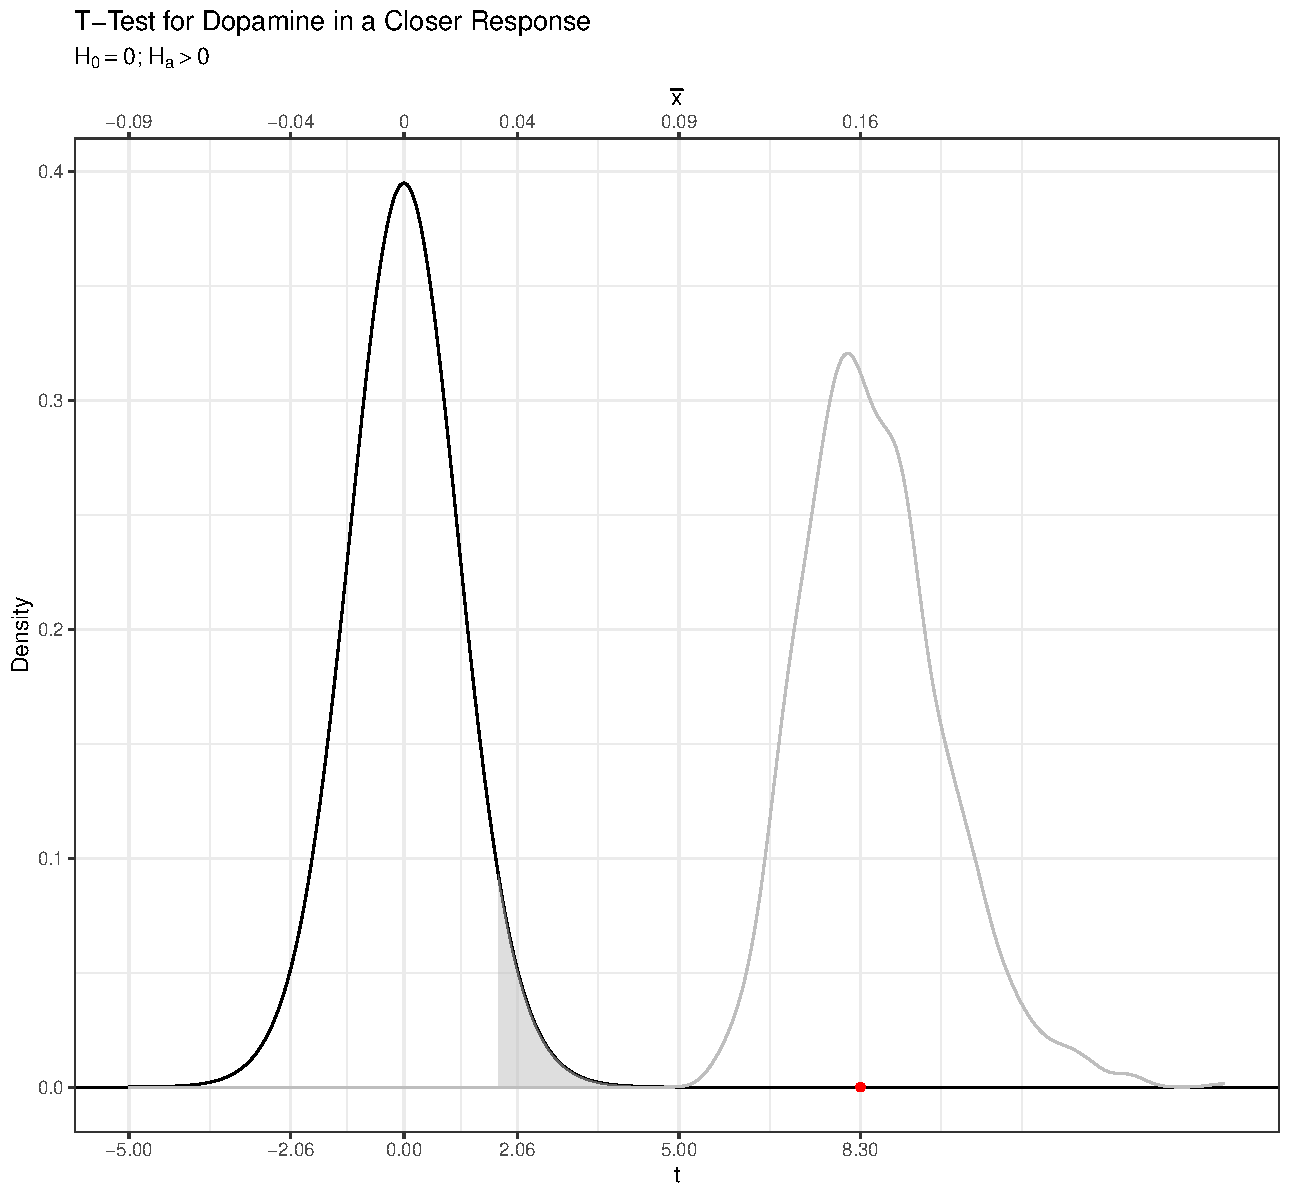
\includegraphics[width=10cm, height=8.5cm]{Rplot.pdf}
\caption{A figure for T-Test for Dopamine in a Closer Response.}
\label{plot1}
\end{figure}

  \item Question 4, part(b).
\begin{figure}[H]
\centering
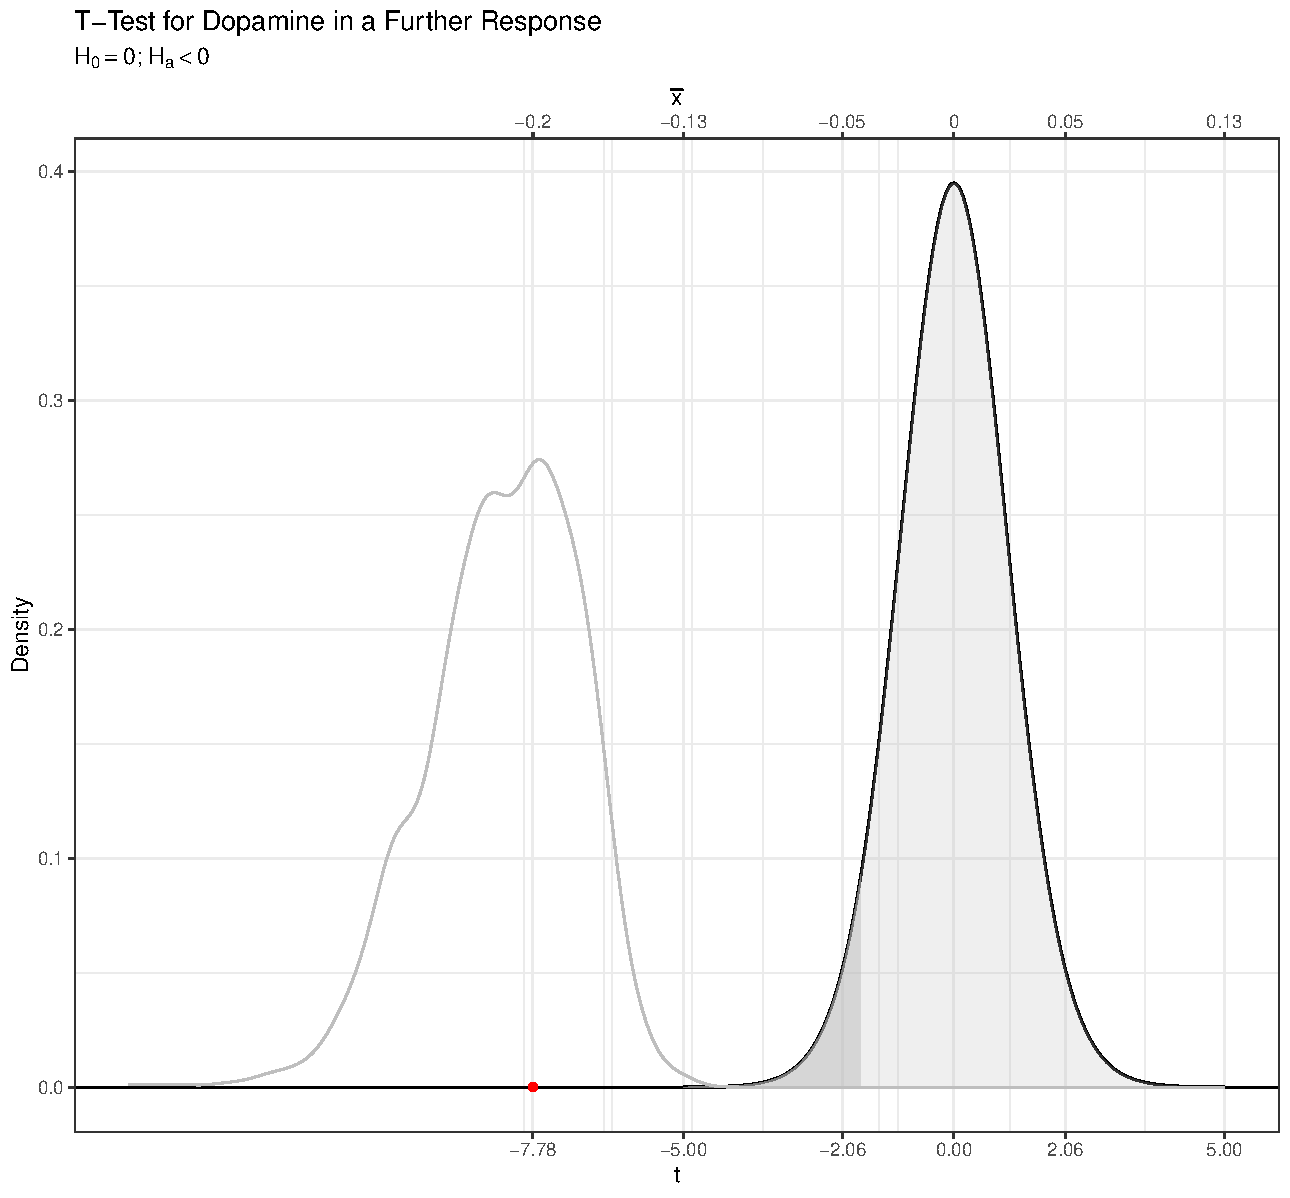
\includegraphics[width=10cm, height=8.5cm]{Rplot01.pdf}
\caption{A figure for T-Test for Dopamine in a Further Response.}
\label{plot2}
\end{figure}

  \item Question 4, part(c).
\begin{figure}[H]
\centering
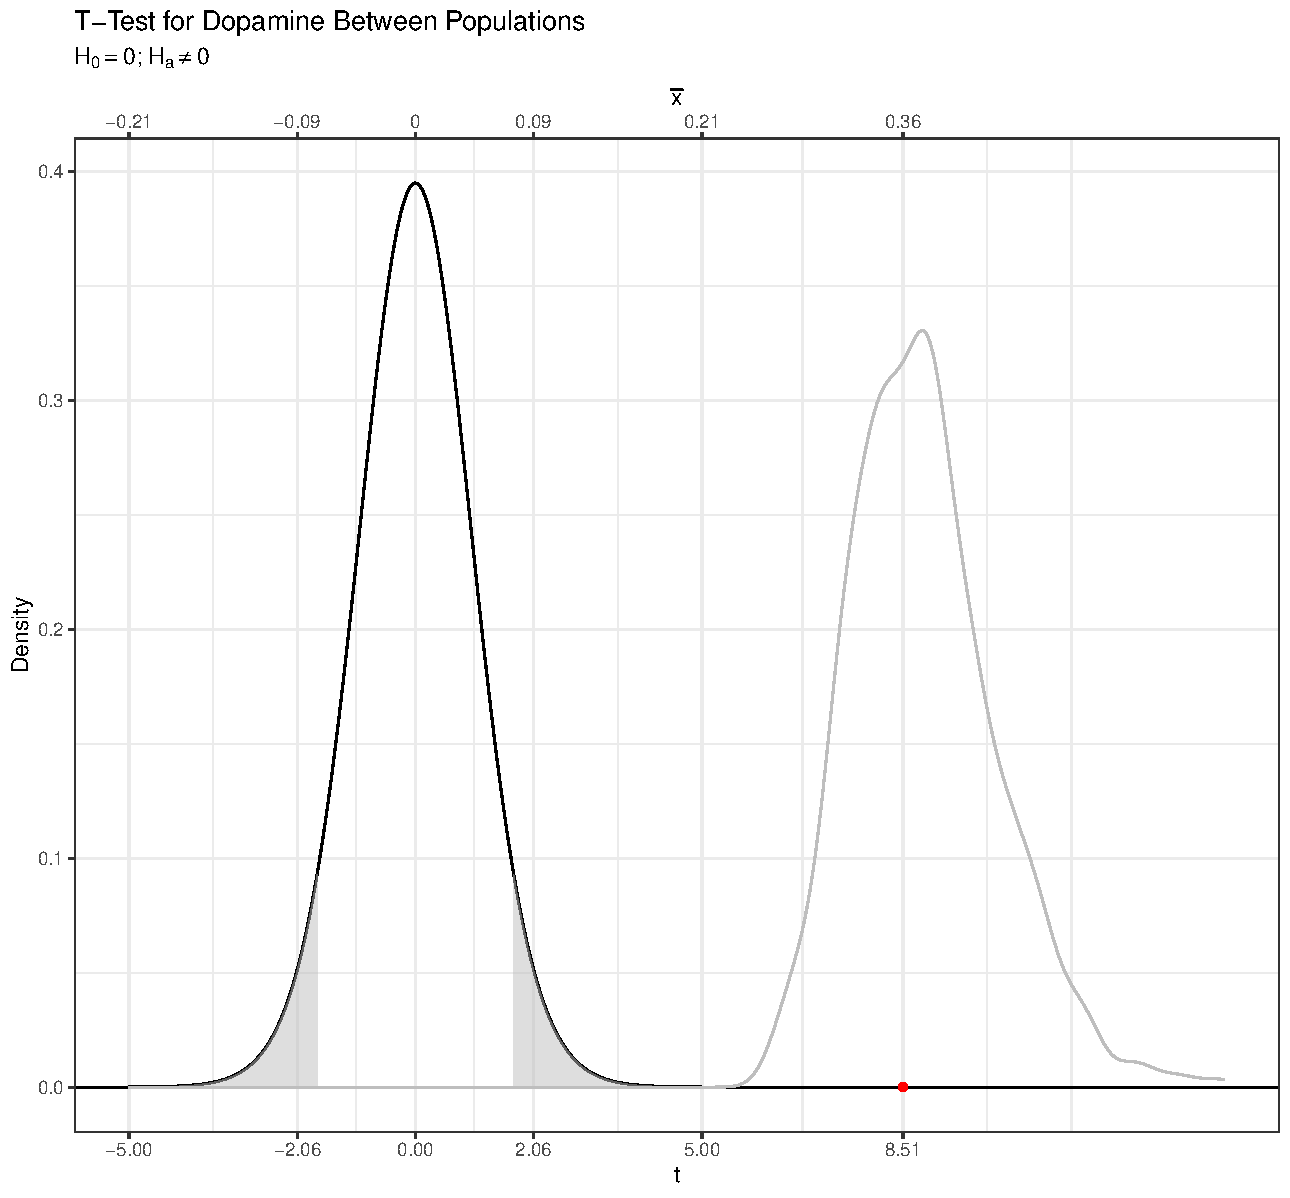
\includegraphics[width=10cm, height=8.5cm]{Rplot02.pdf}
\caption{A figure for T-Test for Dopamine Between Populations.}
\label{plot3}
\end{figure}

\end{enumerate}
\end{enumerate}


\bibliography{bibliography}
\end{document}
